\documentclass{../kin_math}

\header{Elijah Kin}{Homework 11}{AMSC660}
\headrule

\begin{document}

\begin{questions}
  \question
  \begin{enumerate}
    \item Let $\langle \cdot, \cdot \rangle$ be an inner product defined on a vector space $V$. Prove the Cauchy-Schwarz inequality
    \begin{equation}
      |\langle u, v \rangle|^2 \leq \langle u, u \rangle \langle v, v \rangle \quad \forall u, v \in V.
    \end{equation}
    \emph{Hint: Consider the quadratic polynomial}
    \begin{equation}
      p(t) = \langle u + tv, u + tv \rangle, \quad t \in \mathbb{R} \text{ (or $\mathbb{C}$)}.
    \end{equation}
    \emph{Can this polynomial take negative values? Use your answer to conclude what should be the sign of the discriminant if you set $p = 0$.}
    \begin{solution}
      Let $u, v \in V$. Since inner products are non-negative by definition, we have
      \begin{equation*}
        p(t) = \langle u + tv, u + tv \rangle \geq 0
      \end{equation*}
      for all $t \in \mathbb{R}$. Further, using the fact that inner products in linear in their first argument and (conjugate) symmetric,
      \begin{multline*}
        p(t) = \langle u + tv, u + tv \rangle = \langle u, u + tv \rangle + t \langle v, u + tv \rangle \\
        = \langle u + tv, u \rangle + t \langle u + tv, v \rangle = \langle u, u \rangle + t \langle v, u \rangle + t \langle u, v \rangle + t^2 \langle v, v \rangle \\
        = \langle u, u \rangle + 2t \langle u, v \rangle + t^2 \langle v, v \rangle.
      \end{multline*}
      Therefore, we have that
      \begin{equation*}
        \langle u, u \rangle + 2t \langle u, v \rangle + t^2 \langle v, v \rangle \geq 0
      \end{equation*}
      for all $t \in \mathbb{R}$. Hence, in particular it must be true for
      \begin{equation*}
        t^* \coloneqq -\frac{\langle u, v \rangle}{\langle v, v \rangle},
      \end{equation*}
      and so
      \begin{equation*}
        0 \leq p(t^*) = \langle u, u \rangle - 2 \frac{\langle u, v \rangle^2}{\langle v, v \rangle} + \frac{\langle u, v \rangle^2}{\langle v, v \rangle} = \langle u, u \rangle - \frac{\langle u, v \rangle^2}{\langle v, v \rangle}.
      \end{equation*}
      Finally, adding $\frac{\langle u, v \rangle^2}{\langle v, v \rangle}$ and multiplying by $\langle v, v \rangle$ on both sides yields the Cauchy-Schwarz inequality
      \begin{equation*}
        \langle u, v \rangle^2 \leq \langle u, u \rangle \langle v, v \rangle
      \end{equation*}
      as desired.
    \end{solution}
    \item Let $B$ be a real symmetric positive definite $n \times n$ matrix. Use the Cauchy-Schwarz inequality to prove that
    \begin{equation}
      (g^\top B g)(g^\top B^{-1} g) \geq (g^\top g)^2 \quad \forall g \in \mathbb{R}^n.
    \end{equation}
    \begin{solution}
      We first rewrite the right-hand side as a $B$-inner product, noting that
      \begin{equation*}
        (g^\top g)^2 = (g^\top B B^{-1} g)^2 = |\langle g, B^{-1} g \rangle_B|^2
      \end{equation*}
      and so by the Cauchy-Schwarz inequality,
      \begin{multline*}
        (g^\top g)^2 = |\langle g, B^{-1} g \rangle_B|^2 \leq \langle g, g \rangle_B \langle B^{-1} g, B^{-1} g \rangle_B \\
        = (g^\top  B g) ((B^{-1} g)^\top B (B^{-1} g)) = (g^\top B g) (g^\top B^{-1} g)
      \end{multline*}
      as desired.
    \end{solution}
  \end{enumerate}

  \question Consider Newton’s algorithm for solving the trust-region subproblem ([NW], Algorithm 4.3, page 87). Prove that Eq. (4.43) is equivalent to Eq. (4.44) in [NW], i.e., that for
  \begin{equation*}
    \phi(\lambda) = \frac{1}{\Delta} - \left[\sum_{j = 1}^n \frac{(q_j^\top g)^2}{(\lambda_j + \lambda)^2}\right]^{-1 / 2},
  \end{equation*}
  where $(q_j, \lambda_j)$ are the eigenpairs of $B$, the Newton iteration
  \begin{equation*}
    \lambda^{(l + 1)} = \lambda^{(l)} - \frac{\phi(\lambda^{(l)})}{\phi'(\lambda^{(l)})}
  \end{equation*}
  is given by
  \begin{equation*}
    \lambda^{(l + 1)} = \lambda^{(l)} + \left(\frac{\lVert p_l \rVert}{\lVert z_l \rVert}\right)^2 \frac{\lVert p_l \rVert - \Delta}{\Delta},
  \end{equation*}
  where $z_l = L^{-1} p_l$, $p_l = -(B + \lambda^{(l)} I)^{-1} g$, and $L$ is the Cholesky factor of $B + \lambda^{(l)} I$, i.e., $B + \lambda^{(l)} I = LL^\top$. Note: $R = L^\top$ in Algorithm 4.3.

  \emph{Hint: You will need to compute the derivative of $\phi$ and express it in terms of $\lVert p_l \rVert$ and $\lVert (B + \lambda^{(l)} I)^{-1} g \rVert^2$. Also, you will need to use the fact that the Cholesky factor of any SPD matrix $M$ is related to $M^{1 / 2}$ via an orthogonal transformation.}
  \begin{solution}
    We first claim that
    \begin{equation*}
      p_l = -\sum_{j = 1}^n \frac{q_j^\top g}{\lambda_j + \lambda} q_j.
    \end{equation*}
    Since $B$ is symmetric, it has a spectral decomposition $B = Q \Lambda Q^\top$. In particular, we can choose one such that its eigenvectors $\{q_j\}_{j = 1}^n$ are orthonormal. Then
    \begin{equation*}
      B + \lambda^{(l)} I = Q \Lambda Q^\top + \lambda^{(l)} I = Q \Lambda Q^\top + \lambda^{(l)} Q I Q^\top = Q (\Lambda + \lambda^{(l)} I) Q^\top
    \end{equation*}
    and hence
    \begin{equation*}
      p_l = -(B + \lambda^{(l)} I)^{-1} g = -\left(Q (\Lambda + \lambda^{(l)} I) Q^\top\right)^{-1} g = -Q (\Lambda + \lambda^{(l)} I)^{-1} Q^\top g
    \end{equation*}
    meaning
    \begin{equation*}
      p_l = -\sum_{j = 1}^n \frac{q_j^\top g}{\lambda_j + \lambda} q_j.
    \end{equation*}
    Then since the eigenvectors $\{q_j\}_{j = 1}^n$ form an orthonormal basis, this means that
    \begin{equation*}
      \lVert p_l \rVert = \left[\sum_{j = 1}^n \frac{(q_j^\top g)^2}{(\lambda_j + \lambda)^2}\right]^{1 / 2}.
    \end{equation*}
    We now claim that
    \begin{equation*}
      \lVert z_l \rVert = \left[\sum_{j = 1}^n \frac{(q_j^\top g)^2}{(\lambda_j + \lambda)^3}\right]^{1 / 2}.
    \end{equation*}
    From the hint, we know that $L$, the Cholesky factor of $B + \lambda{(l)} I$, can be written as
    \begin{equation*}
      L = Q \sqrt{\Lambda + \lambda^{(l)} I} Q^\top \tilde{Q}
    \end{equation*}
    for some orthogonal matrix $\tilde{Q}$. Hence, $L^{-1} = \tilde{Q}^\top Q (\Lambda + \lambda^{(l)} I)^{-1 / 2} Q^\top$ and so
    \begin{multline*}
      z_l = L^{-1} p_l = (\tilde{Q}^\top Q (\Lambda + \lambda^{(l)} I)^{-1 / 2} Q^\top)(-Q (\Lambda + \lambda^{(l)} I)^{-1} Q^\top g) \\
      = -\tilde{Q}^\top Q (\Lambda + \lambda^{(l)} I)^{-3 / 2} Q^\top g.
    \end{multline*}
    Toward the desired result, recall that multiplication by an orthogonal matrix does not change a vector's norm; let $Q$ be an orthogonal matrix and $x \in \mathbb{R}^n$. Then
    \begin{equation*}
    \lVert Qx \rVert^2 = (Qx)^\top (Qx) = x^\top Q^\top Q x = x^\top x = \lVert x \rVert^2.
    \end{equation*}
    From this fact, we have that
    \begin{multline*}
      \lVert z_l \rVert = \lVert \tilde{Q}^\top Q (\Lambda + \lambda^{(l)} I)^{-3 / 2} Q^\top g \rVert = \lVert Q (\Lambda + \lambda^{(l)} I)^{-3 / 2} Q^\top g \rVert \\
      = \left\lVert \sum_{j = 1}^n \frac{q_j^\top g}{(\lambda_j + \lambda)^{3 / 2}} q_j \right\rVert = \left[\sum_{j = 1}^n \frac{(q_j^\top g)^2}{(\lambda_j + \lambda)^3}\right]^{1 / 2}.
    \end{multline*}
    Hence, we have shown that both
    \begin{equation*}
      \lVert p_l \rVert = \left[\sum_{j = 1}^n \frac{(q_j^\top g)^2}{(\lambda_j + \lambda)^2}\right]^{1 / 2} \text{ and } \lVert z_l \rVert = \left[\sum_{j = 1}^n \frac{(q_j^\top g)^2}{(\lambda_j + \lambda)^3}\right]^{1 / 2}.
    \end{equation*}
    We will now compute $\phi'(\lambda)$ and write it in terms of $\lVert p_l \rVert$ and $\lVert z_l \rVert$, noting that
    \begin{multline*}
      \phi'(\lambda) = \frac{d}{d\lambda} \left[\frac{1}{\Delta} - \left[\sum_{j = 1}^n \frac{(q_j^\top g)^2}{(\lambda_j + \lambda)^2}\right]^{-1 / 2} \right] = \frac{1}{2} \left[\sum_{j = 1}^n \frac{(q_j^\top g)^2}{(\lambda_j + \lambda)^2}\right]^{-3 / 2} \frac{d}{d\lambda} \sum_{j = 1}^n \frac{(q_j^\top g)^2}{(\lambda_j + \lambda)^2} \\
      = -\left[\sum_{j = 1}^n \frac{(q_j^\top g)^2}{(\lambda_j + \lambda)^2}\right]^{-3 / 2} \sum_{j = 1}^n \frac{(q_j^\top g)^2}{(\lambda_j + \lambda)^3} = - \lVert p_l \rVert^{-3} \lVert z_l \rVert^2.
    \end{multline*}
    Finally, we also see that
    \begin{equation*}
      \phi(\lambda) = \frac{1}{\Delta} - \left[\sum_{j = 1}^n \frac{(q_j^\top g)^2}{(\lambda_j + \lambda)^2}\right]^{-1 / 2} = \frac{1}{\Delta} - \frac{1}{\lVert p_l \rVert},
    \end{equation*}
    and hence we have
    \begin{equation*}
      -\frac{\phi(\lambda^{(l)})}{\phi'(\lambda^{(l)})} = \dfrac{\frac{1}{\Delta} - \frac{1}{\lVert p_l \rVert}}{\lVert p_l \rVert^{-3} \lVert z_l \rVert^2} = \dfrac{\frac{\lVert p_l \rVert^{3}}{\Delta} - \lVert p_l \rVert^2}{\lVert z_l \rVert^2} = \dfrac{\lVert p_l \rVert^2}{\lVert z_l \rVert^2} \dfrac{\frac{\lVert p_l \rVert}{\Delta} - 1}{1} = \left(\frac{\lVert p_l \rVert}{\lVert z_l \rVert}\right)^2 \frac{\lVert p_l \rVert - \Delta}{\Delta}
    \end{equation*}
    meaning that Eq. (4.43) and Eq. (4.44) are indeed equivalent.
  \end{solution}

  \question Consider the problem of finding local energy minima of the $\text{LJ}_7$ as in Problem 3 of HW9. Consider the same set of initial conditions: four initial conditions close to its four local minima, and ten random initial conditions.

  Implement the BFGS trust-region method with the dogleg subproblem solver. Compare its performance with the trust-region Newton with the exact subproblem solver implemented in the provided code by creating a table with the number of iterations required to achieve convergence and plotting the graph of $f$ and $\lVert \nabla f \rVert$ against the iteration number for each test case (the four initial conditions close to the minima and one representative random configuration initial condition). Do it for each of the four initial conditions approximating the four local minima and ten random initial conditions. The set of figures to include is the same as for Problem 3 in HW9.

  Comment on the performance of trust-region methods compared to the performance of line-search methods.
  \begin{solution}
    The code and plots for all fourteen runs can be found \href{https://github.com/elijahkin/amsc660/blob/main/hw11/hw11.ipynb}{here}. We supply the plots for model 1 below.
    \begin{figure}
      \centering
      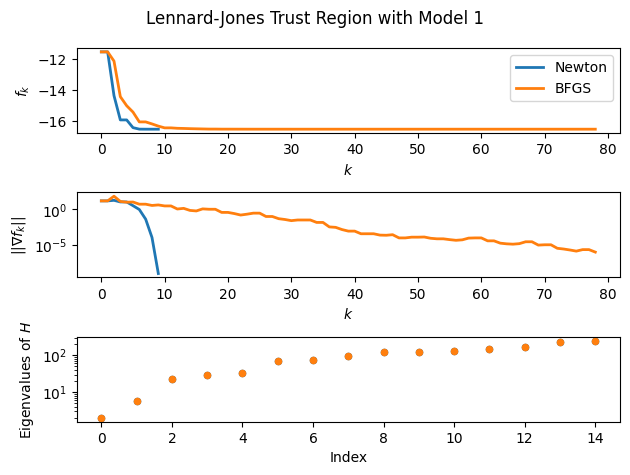
\includegraphics[scale=0.6]{lennard_jones.png}
    \end{figure}
    TODO
  \end{solution}

  \question (Approx. Problem 3.1 from [NW]) Write a code that applies the two algorithms from the previous problem (the trust-region BFGS with the dogleg solver and the trust-region Newton with the exact subspace solver) to the Rosenbrock function as in Problem 4 of HW9:
  \begin{equation}
    f(x, y) = 100(y - x^2)^2 + (1 - x)^2.
  \end{equation}
  Experiment with the same two initial conditions: $(1.2, 1.2)$ and $(-1.2, 1)$.

  Plot the level sets of the Rosenbrock function using the command contour and plot the iterations for each method over it. Plot $\lVert (x_k, y_k) - (x^*, y^*) \rVert$ versus $k$ in the logarithmic scale along the $y$-axis for each method. Compare the performance of the methods.
  \begin{solution}
    \begin{figure}
      \centering
      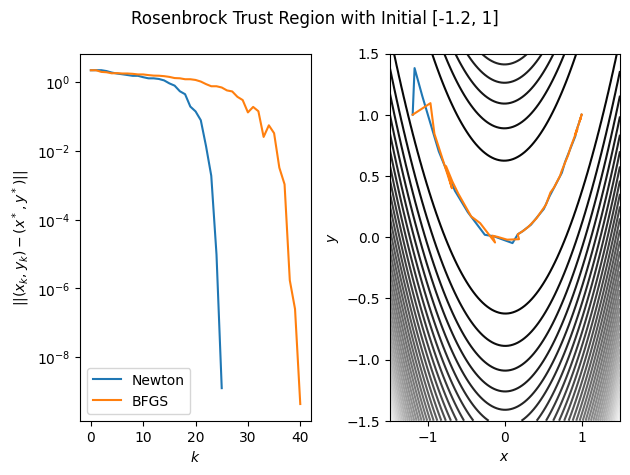
\includegraphics[scale=0.6]{rosenbrock.png}
    \end{figure}
    TODO
  \end{solution}
\end{questions}

\end{document}
